\documentclass[12pt, a4paper]{article}
\setlength{\textheight}{24cm}
\setlength{\textwidth}{16cm}
\setlength{\topmargin}{0cm}
\setlength{\evensidemargin}{0cm}
\setlength{\oddsidemargin}{0cm}
\usepackage[affil-it]{authblk}
\usepackage{graphics}
\usepackage{graphicx}
\usepackage{caption}
\usepackage{float}
\usepackage[british]{babel}
\usepackage{hyperref}
\usepackage{subcaption}
\usepackage{algorithm}
\usepackage{algorithmic}
\date{}
\begin{document}
\title{Comparison of Several FFT Libraries in C/C++}
\author{Philippe Gambron \thanks{\texttt{philippe.gambron{@}stfc.ac.uk}}, Sue Thorne \thanks{\texttt{sue.thorne{@}stfc.ac.uk}}}
\affil{Science and Technology Facilities Council, Hartree Centre, Rutherford Appleton Laboratory, Harwell Campus, Harwell Oxford, OX11 0QZ, United Kingdom}
\maketitle
\begin{abstract}
We compare the performance of several libraries computing FFTs that can be 
called from C or C++ code. In this work, we consider FFTW, MKL, GSL and 
FFTPACK. A benchmarking method was developed in collaboration with CCP-PETMR, 
which we generalised to ensure that this work applied to a wider range of the 
UK's Computational Collaborative Projects and High-End Computing Consortia.
\end{abstract}
\section{Introduction}
Some applications require the computation of the discrete Fourier transform 
(DFT) of large datasets. In such cases, the efficiency of that step can 
become of critical importance. In this report, we compare the performance 
obtained with several libraries that can be called from C or C++:  FFTW \cite{fftw}, MKL \cite{mkl}, GSL \cite{gsl} and FFTPACK \cite{fftpack}.

\section{The Fast Fourier Transform}

The Fourier transform of a discrete signal $x_j, j=1,\ldots,N,$ at uniformally distributed points across a finite domain $[0,N-1]$ in one dimension is given by:
\begin{equation}\label{fourier}
{\cal F}_k=\sum_{j=0}^{N-1} x_j e^{-i\frac{2\pi}{N}kj}, \quad k=1,\ldots,N-1.
\end{equation}

We compute it using the Fast Fourier Transform (FFT) method, which expresses 
the transform recursively as functions of transforms of more sparse subsets 
of the data. The most famous of these methods is the Cooley-Tukey algorithm 
\cite{CT}. The procedure can illustrated by rewriting Equation~\ref{fourier} 
and splitting the sum into two parts with one containing the even values of 
$j$ and the other containing the odd ones multiplied by a phase factor.
\begin{equation}\label{ct}
{\cal F}_k=\sum_{j=0}^{N/2-1}x_{2j}e^{-i\frac{2\pi}{N}2jk}+e^{-i\frac{2\pi}{N}k}\sum_{j=0}^{N/2-1}x_{2j+1}e^{-i\frac{2\pi}{N}2jk}, \quad k=1,\ldots, N-1.
\end{equation}
We can subsequently repeat the procedure by expressing the respective sums as a function of more sparse transforms till we are left only with DFTs of a few data points. This dramatically reduces the number of necessary operations, which become  $\cal{O}\left(N\log(N)\right)$ rather than $\cal{O}\left(N^2\right)$.

We also consider Fourier transforms in more dimensions. For example, in two dimensions, the discrete transform of complex values $z_{j_x j_y}$ located on a grid consisting of $N_x \times N_y$ points is given by:
$$
{\cal F}_{k_x k_y}=\sum_{j_x=0}^{N_x-1} \sum_{j_y=0}^{N_y-1} z_{j_x j_y} e^{-i\left(\frac{2\pi}{N_x} j_x k_x+\frac{2\pi}{N_y} j_y k_y\right)}, \quad k_x=0,\ldots,N_x-1, k_y=0,\ldots,N_y-1.
$$
The inverse of this transform corresponds to:
$$
{\cal F}_{k_x k_y}=\frac{1}{N_xN_y}\sum_{j_x=0}^{N_x-1} \sum_{j_y=0}^{N_y-1} z_{j_x j_y} e^{i\left(\frac{2\pi}{N_x} j_x k_x+\frac{2\pi}{N_y} j_y k_y\right)}, \quad k_x=0,\ldots,N_x-1, k_y=0,\ldots,N_y-1.
$$
  
\section{Benchmark}

The benchmark \cite{code} consists in calculating the FFT of a series of volumes, in 1, 2 or 3 dimensions, 
of real or complex values. The purpose was to mimick a problem submitted to us by the CCP PET-MR 
collaboration \cite{ccppetmr}, within the Software Outlook initiative \cite{softwareoutlook}, who needed to 
take the transform of a series of square complex images. This example is depicted in Figure \ref{benchmark} 
and considered in Section \ref{CCPPETMR}.

\begin{figure}[H]
\captionsetup{width=0.6\textwidth}
\centering
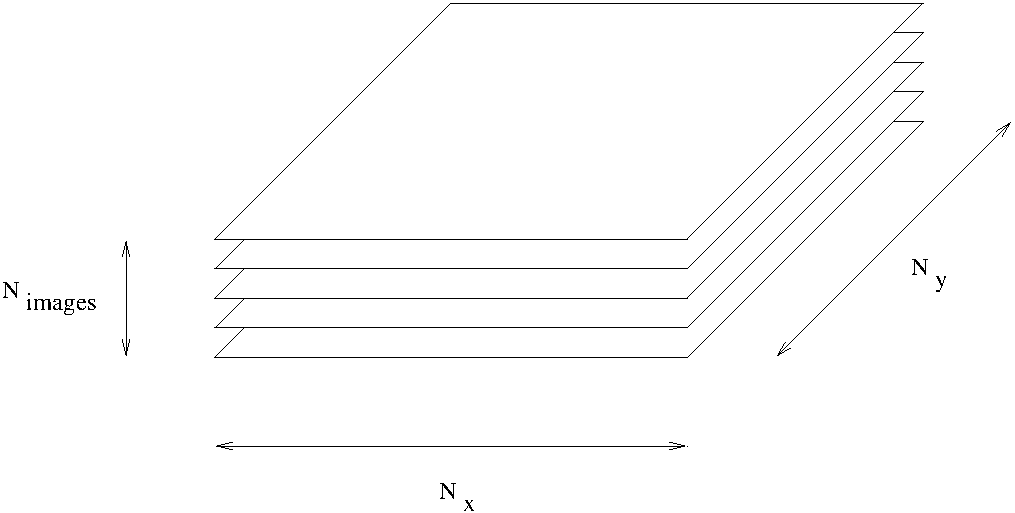
\includegraphics[height=5cm]{benchmark.pdf}
\caption{The benchmark consists in taking the FFT of several images/signals. Each of them is made of real or complex values and can be a simple line, a rectangle or a cuboid.}
\label{benchmark}
\end{figure}

The whole procedure is generalised in Algorithm~\ref{PSEUDOCODE}. We begin by generating $N_s$ signals 
(images) in 1, 2 or 3 dimensions. These can be real or complex values and are sampled at uniformally 
distributed points across the domain. For 1D problems, the sampling is performed at $N$ uniformally 
spaced points across the domain; in 2D the sample points $(j_x,j_y)$ are uniformally distributed 
using a rectangular mesh with $N_x\times N_y$ points; in 3D the domain is discretised using a uniform 
mesh consisting of $N_x\times N_y\times N_z$ grid points. We then initialise the object performing the FFT 
and compute the transform. After this step, we repeat the procedure with the inverse transform, in 
order to compute the error. We will measure the initialisation and execution times of these transforms.
\begin{algorithm}[H]
\centering
\begin{algorithmic}
        \FOR {$i = 0,\ldots, N_s-1$}
        \STATE  $signal[i]=generate\_signal(N_x [,N_y, N_z])$
        \ENDFOR

        \STATE Initialise $FFT$

        \FOR {$i=0,\ldots,N_s-1$}
        \STATE  $transform[i]=FFT(signal[i])$
        \ENDFOR

        \STATE Initialise $inverse\_FFT$

        \FOR {$i=0,\ldots,N_s$}
         \STATE $inverse\_transform[i]=inverse\_FFT(transform[i])$
        \ENDFOR

        \FOR {$i=0,\ldots,N_s-1$}
          \STATE   $error=error+\left\Vert inverse_transform[i]-signal[i]\right\Vert$
        \ENDFOR
\end{algorithmic}
\caption{Pseudocode corresponding to our DFT benchmark}
\label{PSEUDOCODE}
\end{algorithm}

We vary the number of grid points in our benchmark tests. For most of the tests, the domains had 
sides of equal lengths (square or cubic) or were flattened (rectangle or cuboid). These dimensions 
could be powers of 2, products of powers of small integers or prime numbers.

The values appearing in the graphs are the execution time averaged over 10 runs. A certain number 
of bumps or slight unexpected features are apparent. However they were consistently repeated in all 
our measurements. This was also confirmed by the standard deviation of our results, which were always 
quite small and of the order of a few percents of the average value. We chose not to display error 
bars on our graphs since they were so small that they were barely visible. 

\section{Overview of the chosen libraries}
We consider the following libraries computing FFTs: FFTW \cite{fftw}, MKL \cite{mkl}, GSL \cite{gsl} 
and FFTPACK \cite{fftpack} and summarise their attributes in Table~\ref{ffttable}). They can 
perform complex transforms, 
real-to-half-complex ones (and conversely) as well as, in the case of FFTW, real-to-real transforms 
when the signal is odd or even. The half-complex output consists in half as many complex values as 
there were points in the signal, taking advantage of the hermiticity of the Fourier transform of a 
real function.

FFTPACK can compute FFTs in several dimensions but it is written in FORTRAN and all the C or C++ 
wrappers we have found only allow one-dimensional transforms. The GSL library is only designed to 
work in one dimension. However, FFTW and MKL can compute FFTs in several dimensions. They are also 
capable of working in a parallel way, using multithreading and MPI.  
\begin{table}[H]  
\captionsetup{width=1\textwidth}
\begin{tabular}{|l||l|l|l|l|l|}
\hline
& Type & Dim. & Radices & Parallelism & Licence \\
\hline
\hline
FFTW & R$\to$H & Any & 2, 3, 5, 7, 11, 13  & Multithreading  & GPL v2\\
& C$\to$C & & + any with code & MPI &  \\
&  H$\to$R & &  generator & &  \\
& R{\scriptsize (odd/even)}$\to$R & & & &  \\
\hline
MKL  &  R$\to$H & Any & & Multithreading & Proprietary\\
& C$\to$C & & & MPI &  \\
&  H$\to$R & & & &  \\
\hline
GSL  &  R$\to$H & 1 & 2, 3, 5, 6, 7 & - & GPL v3\\
& C$\to$C & & & &  \\
&  H$\to$R & & & &  \\
\hline
FFTPACK  &  R$\to$H  & 1 & & - & GPL v2\\
{\scriptsize (CASA wrapper)} & C$\to$C & & & &  \\
&  H$\to$R & & & &  \\
\hline
\end{tabular}
\caption{Overview of the FFT libraries considered. R stands for real, C for complex, and HC for half-complex.}
\label{ffttable}
\end{table}

\section{Benchmark set-up}
Our benchmark runs were carried out on ARCHER \cite{archer}, the UK National Supercomputing Service. 
It consists of 4920 compute nodes each containing  two 12-core Intel E5-2697 v2 (Ivy Bridge) 
processors and at least 64 GB of RAM. The modules \texttt{gcc/7.2.0} and \\ \texttt{intel/17.0.3.191} 
were loaded. In order to take advantage of multi-threading, the environment variable \texttt{KMP\_AFFINITY} 
must be set to \texttt{disabled}.

Our benchmark was coded in C++ using double-precision reals. More precisely, we used version 3.3.8 
of FFTW, version 17.0.3 of MKL and version 2.5 of GSL. Note that we used our own version of Boost, 
FFTW and GSL because the version of Boost present on the system was lacking certain libraries and 
we wanted to use the most recent versions of FFTW and GSL. The benchmark was compiled with the flags
 \texttt{-std=c++1z -O3  -fopenmp   -lm -lfftw3 -lfftw3\_threads -lgslcblas -lgsl -lboost\_system -lboost\_chrono\\-liomp5 -lmkl\_core -lmkl\_intel\_thread -lmkl\_intel\_lp64  -lcasa\_scimath \\-llapack}.

Since FFTPACK was written in FORTRAN, we have resorted to the C++ wrapper provided by CASA, the 
radioastronomy package \cite{casa}. This is straightforward to install on Debian-like systems, 
such as the one used by CCP PET-MR in their virtual environment, where CASA can be installed 
using the package manager. However, including the headers and linking with the libraries was 
not possible with the version of CASA distributed by the National Radio Astronomy Observatory. 
As a consequence, this was quite difficult to set up on ARCHER and required the use of libraries 
provided by an old version of Debian to match those available on the system. For this reason, it 
was also necessary to use an older version of CASA, 2.4.0.


\section{Effect of the domain size in one dimension}\label{PERFORMANCE1D}

In this section, we compare the performance of each library, in one dimension. 
Our example corresponds to the pseudocode in Algorithm~\ref{PSEUDOCODE}. We have 
used a single signal ($N_s=1$) and the number of grid points, $N,$ is set to be either a power of 2, 
an integer number of the form $2^j\ 3^k\ 5^l\ 7^m$ or a prime number. The latter are chosen to be 
close to the corresponding power of 2 (Table~\ref{SIZES1D}).
\begin{table}[H]
\captionsetup{width=0.8\linewidth}
\centering
\begin{tabular}{|l|l|l|}
  \hline
  \multicolumn{3}{|c|}{$N$}\\
  \hline
  \hline
Powers of 2 & prod. pow. int. & primes\\ \hline
$2^8=256$	 & $2^2\ 3^2\ 5\ 7=210$	     & 257  \\ \hline
$2^{10}=1024$	 & $2^2\ 3^2\ 5\ 7=1260$	     & 1021  \\ \hline
$2^{12}=4096$	 & $2\ 3^2\ 5\ 7=4410$	     & 4093 \\ \hline
$2^{14}=16384$	 & $2\ 3^2\ 5^3\ 7=15750$	     & 16381 \\ \hline
$2^{16}=65536$	 & $2\ 3^3\ 5^2\ 7^2=66150$      & 65521 \\ \hline
$2^{18}=262144$	 & $2\ 3\ 5^3\ 7^3=257250$       & 262139 \\ \hline
$2^{20}=1048576$  & $2\ 3^2\ 5^2\ 7^4=1080450$    & 1048573 \\ \hline
$2^{22}=4194304$  & $2^2\ 3^2\ 5^2 7^4=4321800$  &	\\ \hline
$2^{24}=16777216$ & $2^3\ 3^2\ 5^4\ 7^3=15435000$ &	\\ \hline
$2^{26}=67108864$ & $2^3\ 3^3\ 5^3\ 7^4=64827000$ &\\ \hline
\end{tabular}
\caption{Number of points used for the benchmark in one dimension}\label{SIZES1D}
\end{table}


 We run our benchmarks with both real and complex values signals and use the DFT libraries 
FFTW (Figure~\ref{1DFFTW}), MKL (Figure~\ref{1DMKL}), GSL (Figure~\ref{1DGSL}) and FFTPACK 
(Figure~\ref{1DFFTPACK}). For each library, we compare the effect of using the different 
classes of $N.$ We then compare the different libraries for powers of 2 (Figure~\ref{1DPOW2}) and, 
in general, (Figure~\ref{1D}). In each of these cases, we have plotted the wallclock initialisation time and 
wallclock forward DFT execution times as a function of $N.$ We will investigate the effect of parallelism in 
Section~\ref{PARALLELISM}. As a consequence, for the moment, we will run all those benchmarks s
erially, as a single process containing a single thread.


\subsection{1D FFTW}
Analysing the performance of FFTW in Figure~\ref{1DFFTW}, the initialisation time for real input 
signals is similat for $N$ a power of 2 and values of $N$ that can be factored into a product of 
small integers: for larger values of $N,$ it increases proportionally to a power of $N.$ For 
values of $N$ greater than $2^{14},$ the initialisation times for prime values of $N$ are at 
least 20 times higher than the other classes of $N.$ The behaviour of the initialisation times 
is different when the signal is complex-valued. Namely, when $N$ is a power of 2, the initialisation 
time flattens out when $N>10^6.$ Initialisation times are faster for complex input compared to real 
input: when $N$ can be factored into a product of small integers, the difference is approximately a 
factor of 2. Compairing DFT execution times for real and complex input signals, the behaviour is very 
similar but the complex runs are roughly 2 times slower than when the signal is real-valued and $N$ 
is a power of 2 or the product of small integers. When $N$ is prime, the execution times are almost 
identical for real and complex signals. 




 
\begin{figure}[htb]
\captionsetup{width=0.8\linewidth}
\centering
\begin{subfigure}{.5\textwidth}
\centering
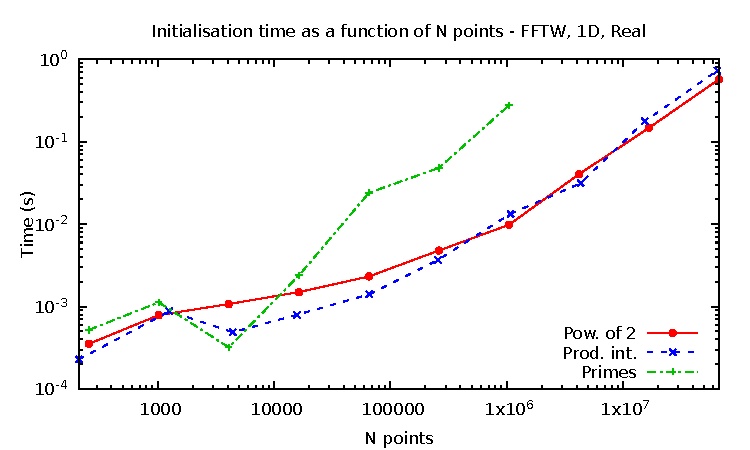
\includegraphics[width=.9\linewidth]{graphs/1d-fftw-init-r.pdf}
\caption{Intialisation (real)}
\label{1DFFTWRI}
\end{subfigure}%
\begin{subfigure}{.5\textwidth}
\centering
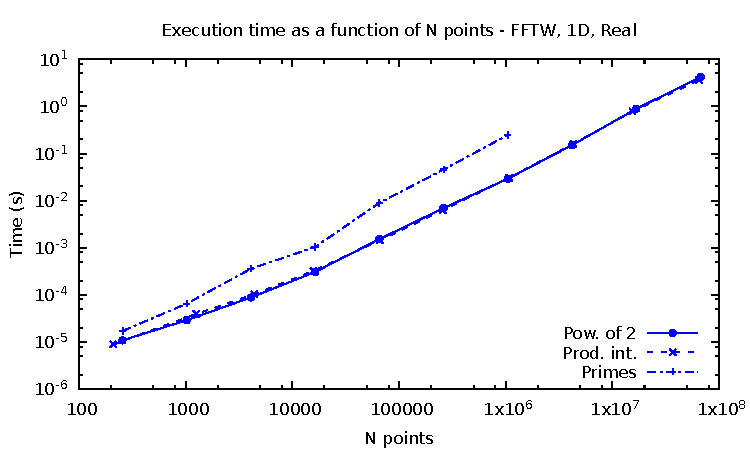
\includegraphics[width=.9\linewidth]{graphs/1d-fftw-exec-r.pdf}
\caption{Execution (real)}
\label{1DFFTWR}
\end{subfigure}\\
\begin{subfigure}{.5\textwidth}
\centering
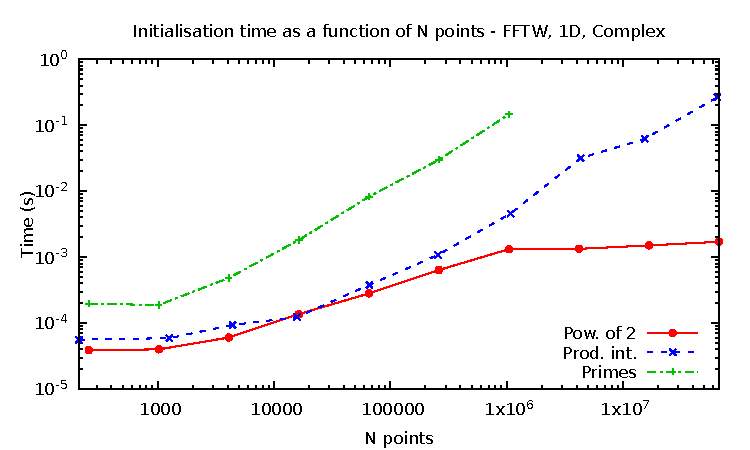
\includegraphics[width=.9\linewidth]{graphs/1d-fftw-init-c.pdf}
\caption{Intialisation (complex)}
\label{1DFFTWCI}
\end{subfigure}%
\begin{subfigure}{.5\textwidth}
\centering
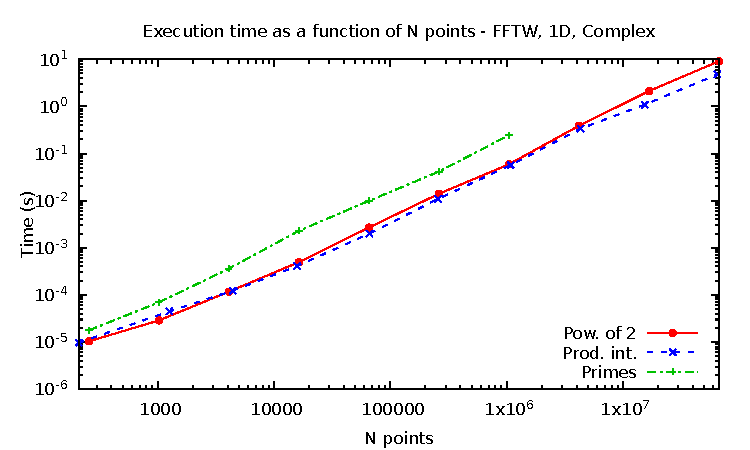
\includegraphics[width=.9\linewidth]{graphs/1d-fftw-exec-c.pdf}
\caption{Execution (complex)}
\label{1DFFTWC}
\end{subfigure}
\caption{Initialisation and execution times as a function of the number of points (1 dimension, FFTW)}
\label{1DFFTW}
\end{figure}

\subsection{1D MKL}
Figure~\ref{1DMKL} compares the initialisation and DFT execution times for the MKL library. When the 
signal is real-valued, there is little difference in initialisation times for $N$ a power of 2 and $N$ 
a product of small integers. Additionally, the initialisation time is increasing proportionally to a 
power of the problem size. When $N$ is prime and the signal is real-valued, there is only a relatively 
small increase in intialisation time as the problem size increases. When the signal contains complex 
values, the initialisation time is roughly 1.5 times larger for $N$ a product of small integers 
compared to $N$ being a power of 2. Additionally, for these cases, the initialisation time is roughly 
an order of magnitude smaller than when the signal has real entries.

The DFT execution times for $N$ a power of 2 or product of small integers are highly correlated to 
problem size with execution times for real input taking roughly twice the time of signals with complex 
entries. When $N$ is prime, the DFT execution time is 2.2 times longer when the signal is real instead 
of complex.

\begin{figure}[htb]
\captionsetup{width=0.8\linewidth}
\centering
\begin{subfigure}{.5\textwidth}
\centering
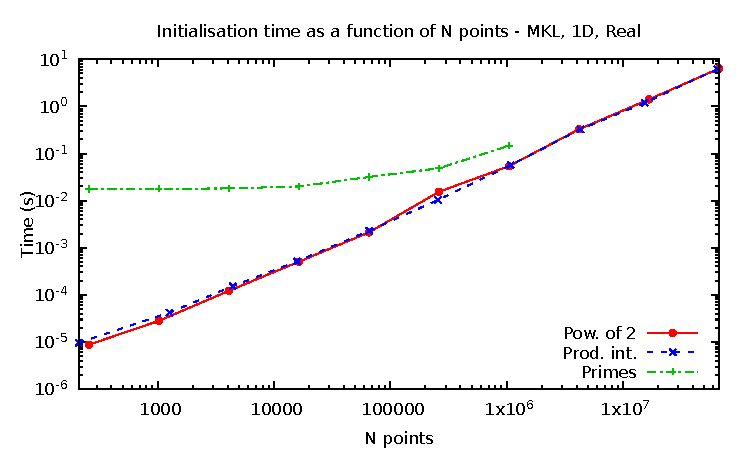
\includegraphics[width=.9\linewidth]{graphs/1d-mkl-init-r.pdf}
\caption{Intialisation (real)}
\label{1DMKLRI}
\end{subfigure}%
\begin{subfigure}{.5\textwidth}
\centering
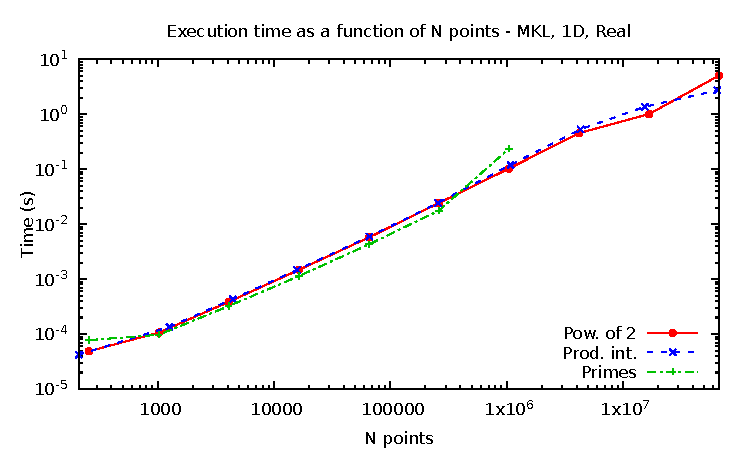
\includegraphics[width=.9\linewidth]{graphs/1d-mkl-exec-r.pdf}
\caption{Execution (real)}
\label{1DMKLR}
\end{subfigure}\\
\begin{subfigure}{.5\textwidth}
\centering
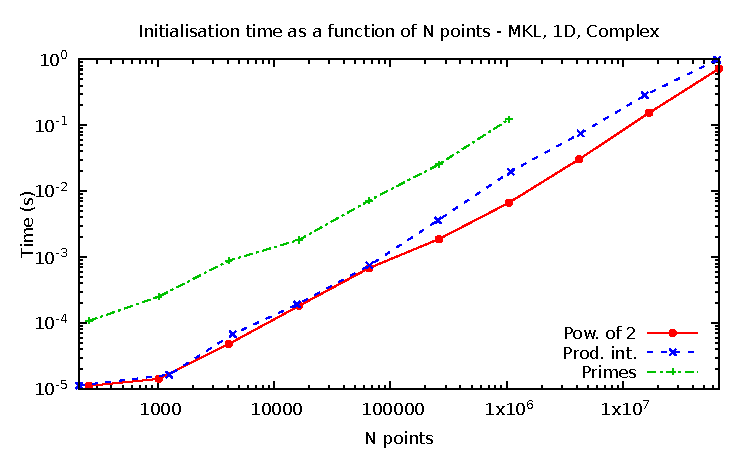
\includegraphics[width=.9\linewidth]{graphs/1d-mkl-init-c.pdf}
\caption{Intialisation (complex)}
\label{1DMKLCI}
\end{subfigure}%
\begin{subfigure}{.5\textwidth}
\centering
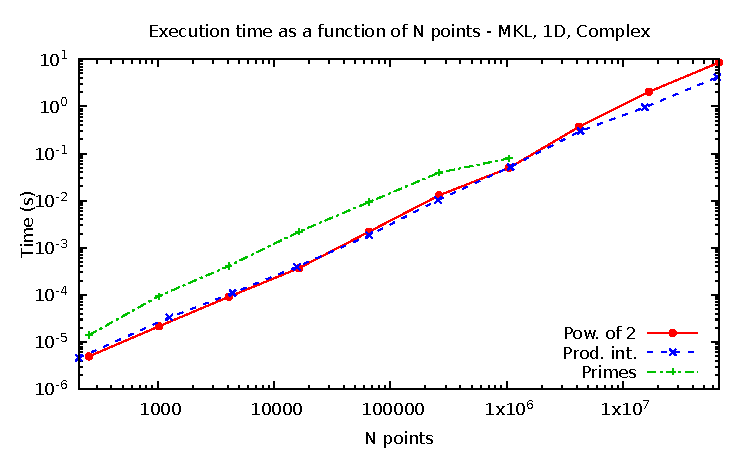
\includegraphics[width=.9\linewidth]{graphs/1d-mkl-exec-c.pdf}
\caption{Execution (complex)}
\label{1DMKLC}
\end{subfigure}\\
\caption{Initialisation and execution times as a function of the number of points (1 dimension, MKL)}
\label{1DMKL}
\end{figure}

\subsection{1D GSL and FFTPACK}
As with the FFTW and MKL libraries, the initialisation times for GSL, Figure~\ref{1DGSL}, have 
differing behaviours for real and complex signals. For complex signals, there is little difference 
in initialisation time for the different classes of $N$ and the time is proportional to a power of 
the problem size. When the signal is real, rather surprisingly, the initialisation time is smallest 
when $N$ is prime and the times for the other cases are roughly those for corresponding complex 
signals. For real-valued signals with prime values of $N,$ the DFT execution time increases at a 
rate proportional to $N^2.$ For complex signals with $N$ prime, there is a much slower increase 
with respect to execution time and the times are roughly 2.5 times those of the other classes of 
$N$ considered.

The general behaviours of the GSL and FFTPACK (Figure~\ref{1DFFTPACK}) libraries are similar.  

\begin{figure}[htb]
\captionsetup{width=0.8\linewidth}
\centering
\begin{subfigure}{.5\textwidth}
\centering
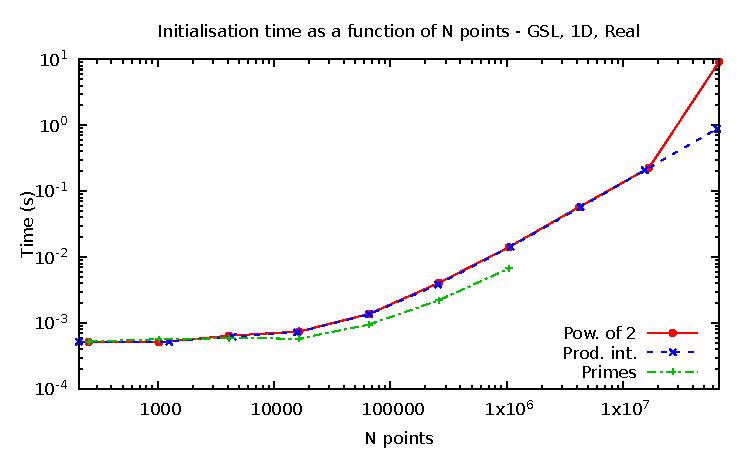
\includegraphics[width=.9\linewidth]{graphs/1d-gsl-init-r.pdf}
\caption{Intialisation (real)}
\label{1DGSLRI}
\end{subfigure}%
\begin{subfigure}{.5\textwidth}
\centering
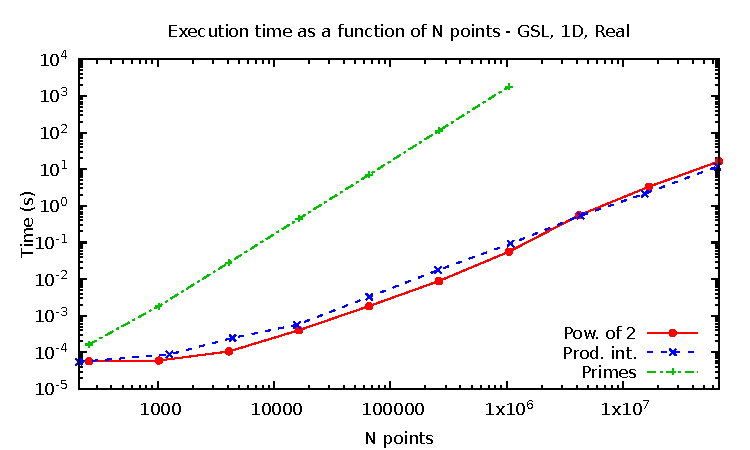
\includegraphics[width=.9\linewidth]{graphs/1d-gsl-exec-r.pdf}
\caption{Execution (real)}
\label{1DGSLR}
\end{subfigure}\\
\begin{subfigure}{.5\textwidth}
\centering
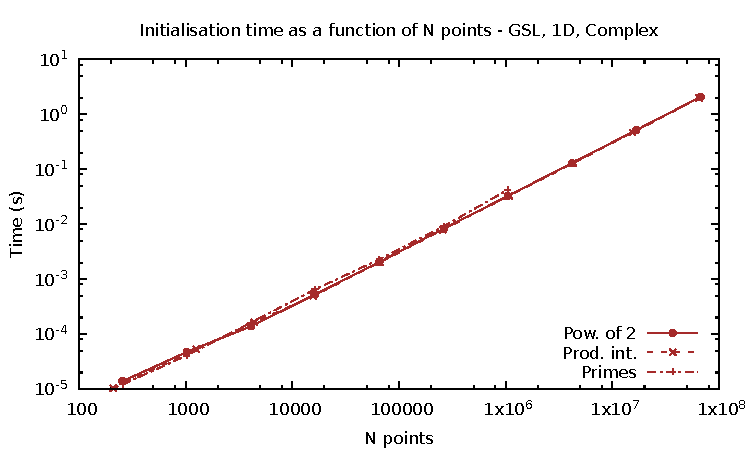
\includegraphics[width=.9\linewidth]{graphs/1d-gsl-init-c.pdf}
\caption{Intialisation (complex)}
\label{1DGSLCI}
\end{subfigure}%
\begin{subfigure}{.5\textwidth}
\centering
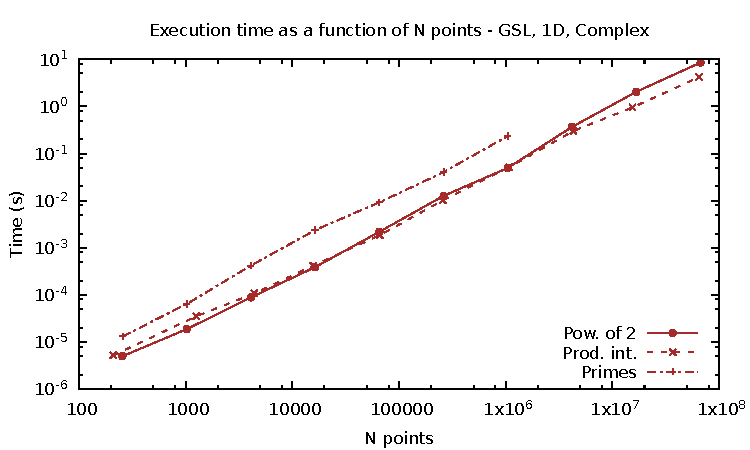
\includegraphics[width=.9\linewidth]{graphs/1d-gsl-exec-c.pdf}
\caption{Execution (complex)}
\label{1DGSLC}
\end{subfigure}
\caption{Initialisation and execution times as a function of the number of points (1 dimension, GSL)}
\label{1DGSL}
\end{figure}

\begin{figure}[H]
\captionsetup{width=0.8\linewidth}
\centering
\begin{subfigure}{.5\textwidth}
\centering
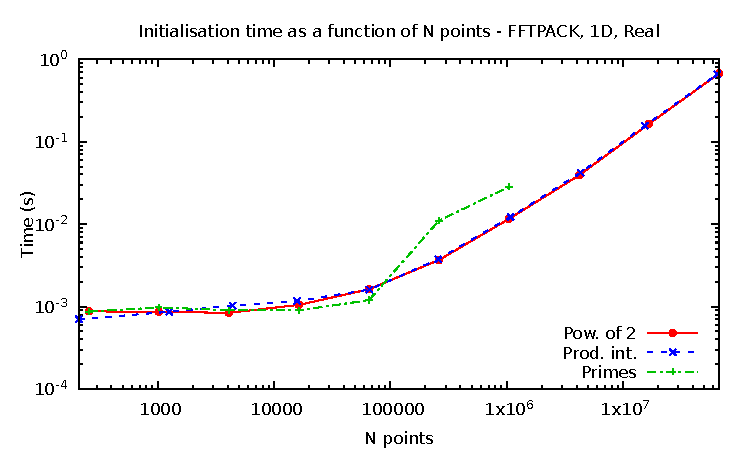
\includegraphics[width=.9\linewidth]{graphs/1d-fftpack-init-r.pdf}
\caption{Intialisation (real)}
\label{1DFFTPACKRI}
\end{subfigure}%
\begin{subfigure}{.5\textwidth}
\centering
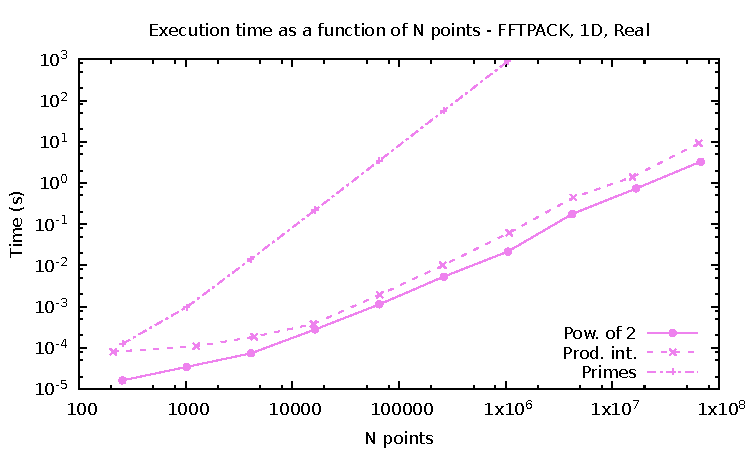
\includegraphics[width=.9\linewidth]{graphs/1d-fftpack-exec-r.pdf}
\caption{Execution (real)}
\label{1DFFTPACKR}
\end{subfigure}\\
\begin{subfigure}{.5\textwidth}
\centering
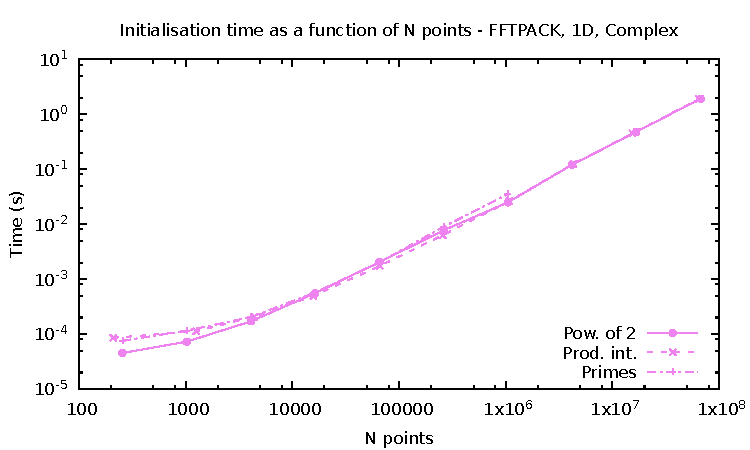
\includegraphics[width=.9\linewidth]{graphs/1d-fftpack-init-c.pdf}
\caption{Intialisation (complex)}
\label{1DFFTPACKCI}
\end{subfigure}%
\begin{subfigure}{.5\textwidth}
\centering
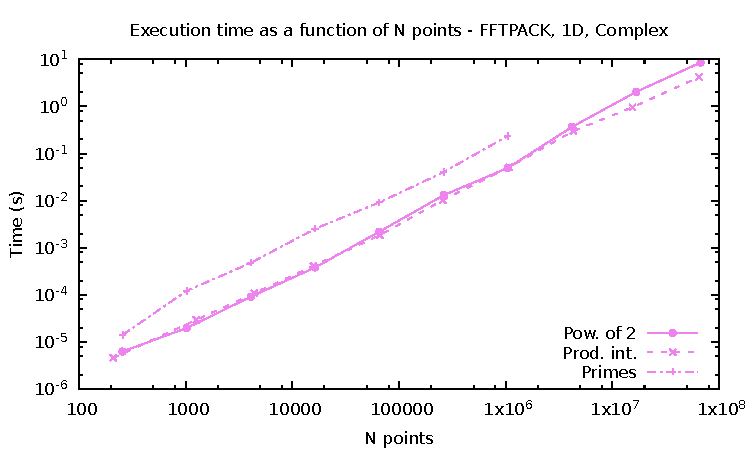
\includegraphics[width=.9\linewidth]{graphs/1d-fftpack-exec-c.pdf}
\caption{Execution (complex)}
\label{1DFFTPACKC}
\end{subfigure}
\caption{Initialisation and execution times as a function of the number of points (1 dimension, FFTPACK)}
\label{1DFFTPACK}
\end{figure}


\subsection{Comparison libraries for 1D benchmarks}
We also compared the libraries among themselves for powers of 2 (Figure~\ref{1DPOW2}) and all the 
classes of $N$ considered (Figure~\ref{1D}).  No clear winner emerges from our measurements with 
respect to DFT time. For 
real signals, FFTW and FFTPACK are the fastest for powers of 2 while, for products of powers of small 
integers, it is FFTW and, in the case of prime numbers, FTTW and MKL. For complex signals, the 
performances obtained with each library are quite close except with products of powers small integers 
where FFTW is the most efficient. We also notice that the performance with primes is significantly worse, 
with real numbers, in the cases of GSL and FFTPACK. As a conclusion, in one dimension, FFTW seems to be 
the best all-rounder.

\begin{figure}[H]
\captionsetup{width=0.8\linewidth}
\centering
\begin{subfigure}{.5\textwidth}
\centering
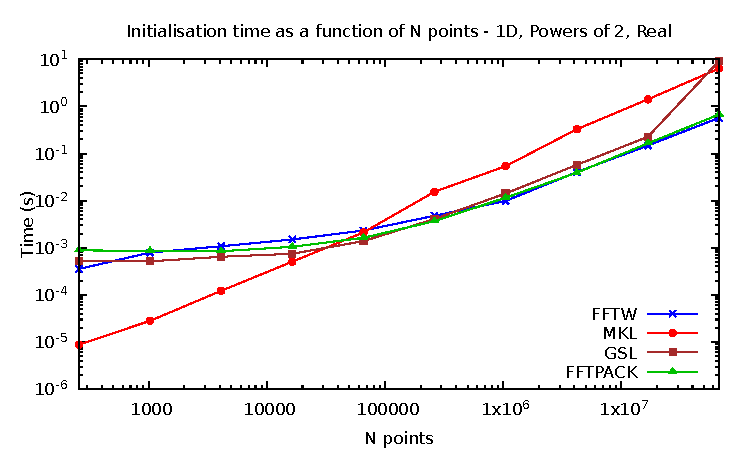
\includegraphics[width=.9\linewidth]{graphs/1d-pow2-init-r.pdf}
\caption{Intialisation (real)}
\label{1DPOW2RI}
\end{subfigure}%
\begin{subfigure}{.5\textwidth}
\centering
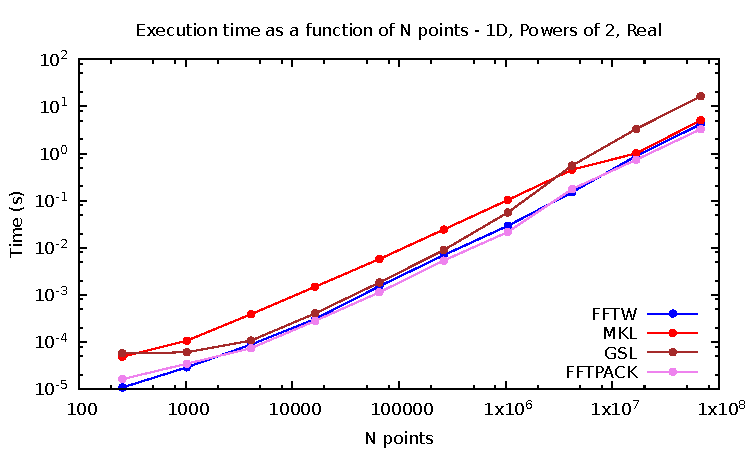
\includegraphics[width=.9\linewidth]{graphs/1d-pow2-exec-r.pdf}
\caption{Execution (real)}
\label{1DPOW2R}
\end{subfigure}\\
\begin{subfigure}{.5\textwidth}
\centering
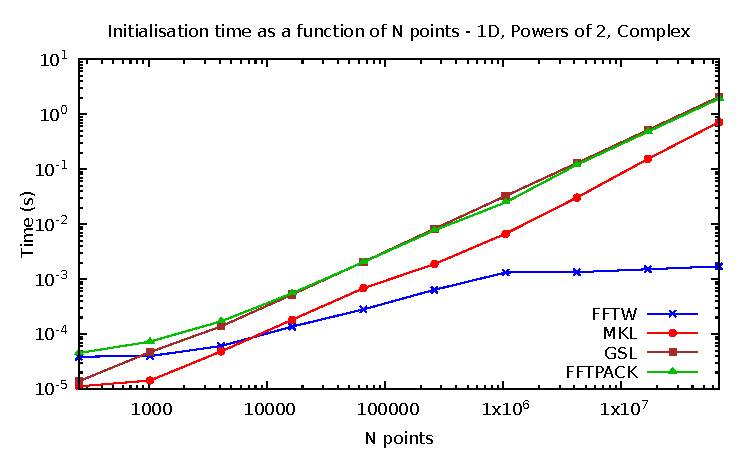
\includegraphics[width=.9\linewidth]{graphs/1d-pow2-init-c.pdf}
\caption{Intialisation (complex)}
\label{1DPOW2CI}
\end{subfigure}%
\begin{subfigure}{.5\textwidth}
\centering
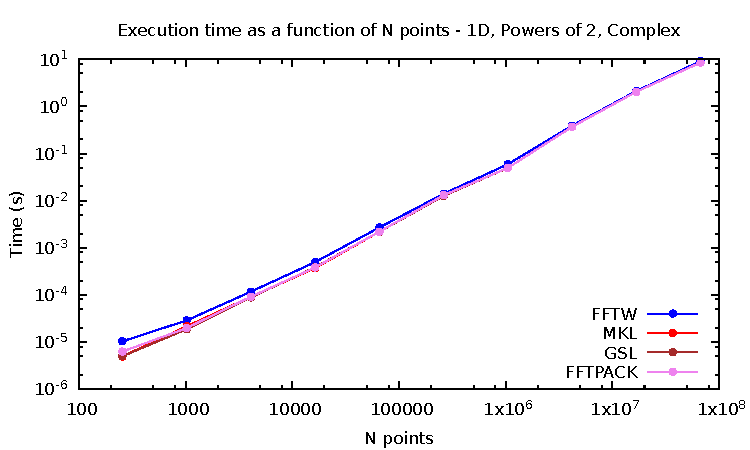
\includegraphics[width=.9\linewidth]{graphs/1d-pow2-exec-c.pdf}
\caption{Execution (complex)}
\label{1DPOW2C}
\end{subfigure}
\caption{Initialisation and execution times as a function of the number of points (1 dimension, powers of 2)}
\label{1DPOW2}
\end{figure}

\begin{figure}[H]
\captionsetup{width=0.8\linewidth}
\centering
\begin{subfigure}{.5\textwidth}
\centering
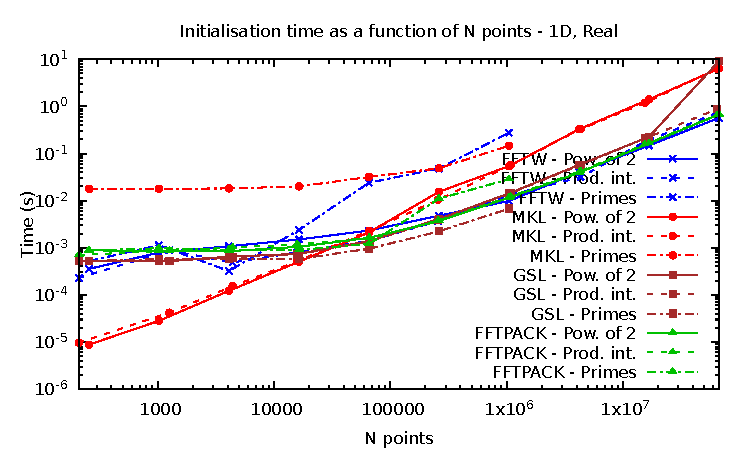
\includegraphics[width=.9\linewidth]{graphs/1d-init-r.pdf}
\caption{Intialisation (real)}
\label{1DRI}
\end{subfigure}%
\begin{subfigure}{.5\textwidth}
\centering
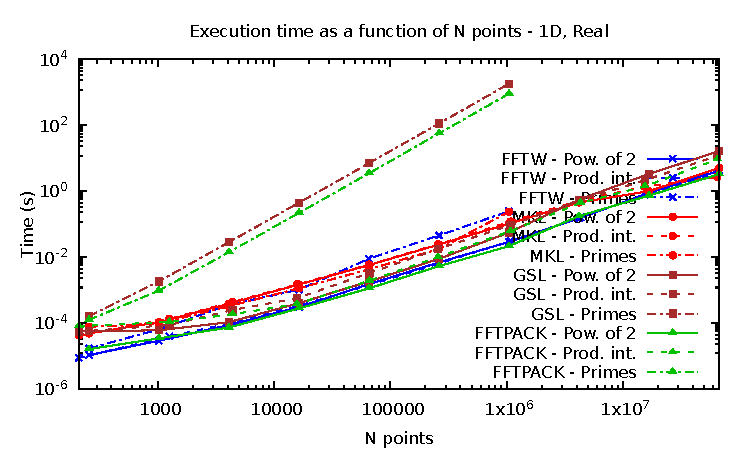
\includegraphics[width=.9\linewidth]{graphs/1d-exec-r.pdf}
\caption{Execution (real)}
\label{1DR}
\end{subfigure}\\
\begin{subfigure}{.5\textwidth}
\centering
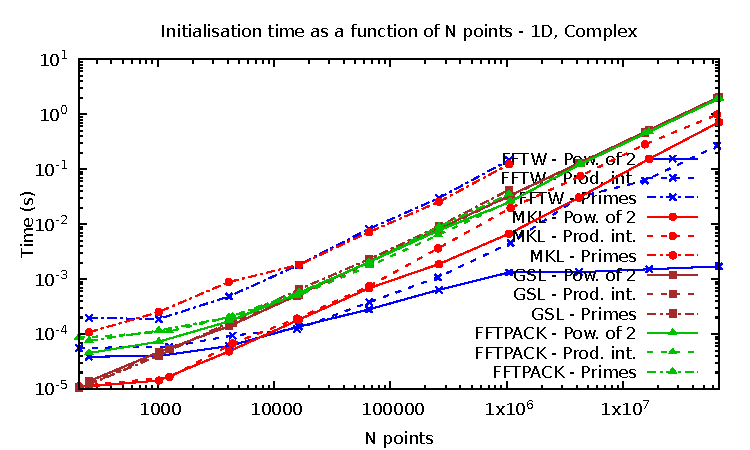
\includegraphics[width=.9\linewidth]{graphs/1d-init-c.pdf}
\caption{Intialisation (complex)}
\label{1DCI}
\end{subfigure}%
\begin{subfigure}{.5\textwidth}
\centering
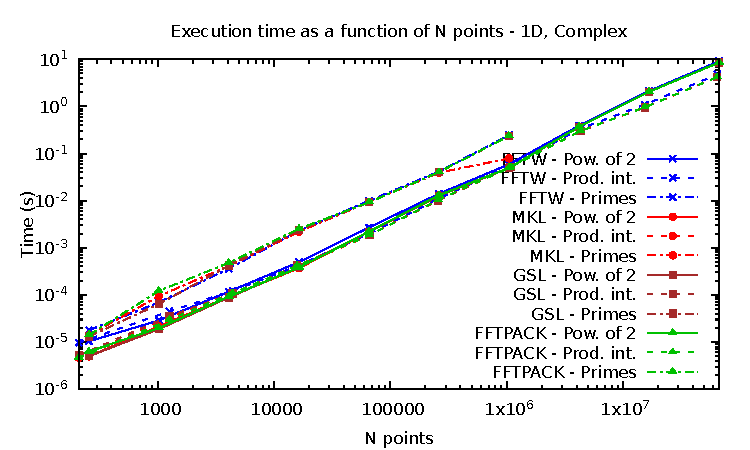
\includegraphics[width=.9\linewidth]{graphs/1d-exec-c.pdf}
\caption{Execution (complex)}
\label{1DC}
\end{subfigure}
\caption{Initialisation and execution times as a function of the number of points (1 dimension)}
\label{1D}
\end{figure}

\section{Effect of the domain size in two dimensions}\label{PERFORMANCE2D}

In this section, we measure the performance obtained in two dimensions following the same procedure as in Section \ref{PERFORMANCE1D}. However, only FFTW and MKL work in this case (Figure~\ref{2DFFTW} and \ref{2DMKL}). We study only a square domain. We will consider asymmetrical domains in Section \ref{FLATNESS}. 

We begin by comparing the performance obtained with numbers of points that are a power of 2, the product of powers of small integers or a prime number. These numbers are chosen as in Section \ref{PERFORMANCE1D} and we endeavoured make the total number of points vary within a similar range. The dimensions we chose appear in the Table \ref{SIZES2D}.

\begin{table}[H]
\captionsetup{width=0.8\linewidth}
\centering
\begin{tabular}{|l|l|l|}
  \hline
  \multicolumn{3}{|c|}{$N_x=N_y$}\\
  \hline
  \hline
Powers of 2 & prod. pow. int. & primes\\ \hline
$2^9=512$ & $2^3\ 3^2\ 7=504$ & 509\\ \hline
$2^{10}=1024$ & $3\ 7^3=1029$ & 1021\\ \hline
$2^{11}=2048$ & $2\ 3\ 7^3=2058$ & 2027\\ \hline
$2^{12}=4096$ & $2^2\ 3\ 7^3=4116$ & 4049\\ \hline
$2^{13}=8192$ & $2^3\ 3\ 7^3=8232$ & 8123\\ \hline
\end{tabular}
\caption{Number of points on the side of the square}\label{SIZES2D}
\end{table}


 As in one dimension (Section \ref{PERFORMANCE1D}), we obtain the best performance when the number of elements on each side is a power of 2 or the product of powers of small integers rather than a prime number. We observe that, in 2 dimensions, the MKL library is the most efficient.
 

\begin{figure}[H]
\captionsetup{width=0.8\linewidth}
\centering
\begin{subfigure}{.5\textwidth}
\centering
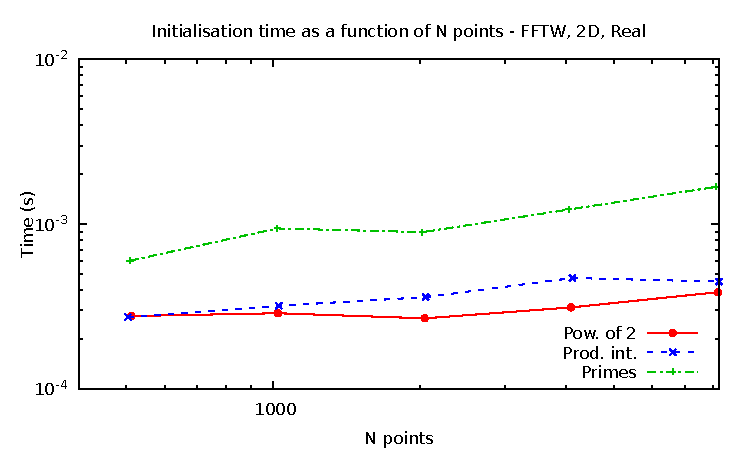
\includegraphics[width=.9\linewidth]{graphs/2d-fftw-init-r.pdf}
\caption{Intialisation (real)}
\label{2DFFTWRI}
\end{subfigure}%
\begin{subfigure}{.5\textwidth}
\centering
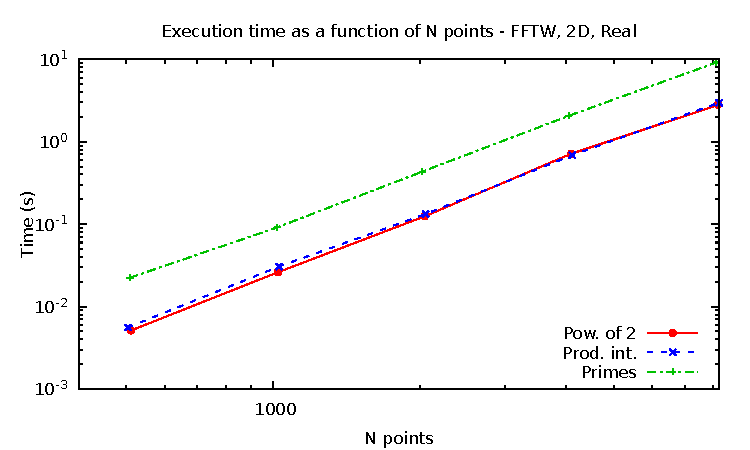
\includegraphics[width=.9\linewidth]{graphs/2d-fftw-exec-r.pdf}
\caption{Execution (real)}
\label{2DFFTWR}
\end{subfigure}\\
\begin{subfigure}{.5\textwidth}
\centering
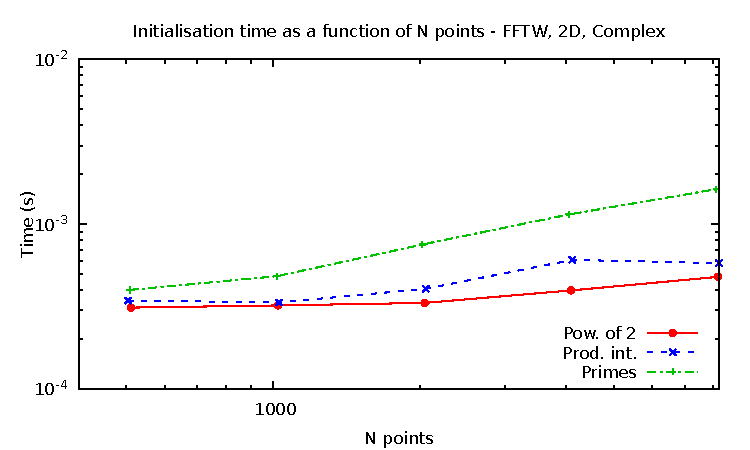
\includegraphics[width=.9\linewidth]{graphs/2d-fftw-init-c.pdf}
\caption{Intialisation (complex)}
\label{2DFFTWCI}
\end{subfigure}%
\begin{subfigure}{.5\textwidth}
\centering
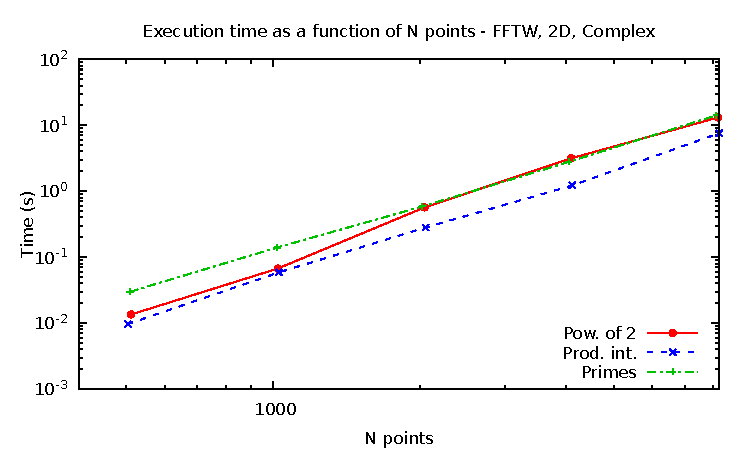
\includegraphics[width=.9\linewidth]{graphs/2d-fftw-exec-c.pdf}
\caption{Execution (complex)}
\label{2DFFTWC}
\end{subfigure}
\caption{Initialisation and execution times as a function of the side of the square (2 dimensions, FFTW)}
\label{2DFFTW}
\end{figure}
\begin{figure}[H]
\captionsetup{width=0.8\linewidth}
\centering
\begin{subfigure}{.5\textwidth}
\centering
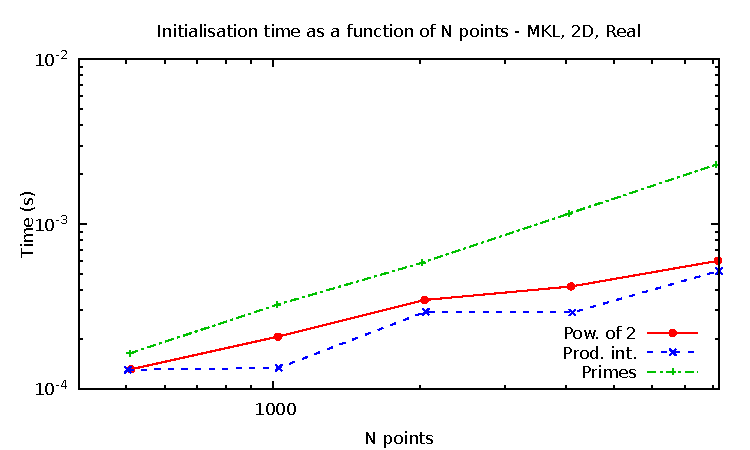
\includegraphics[width=.9\linewidth]{graphs/2d-mkl-init-r.pdf}
\caption{Intialisation (real)}
\label{2DMKLRI}
\end{subfigure}%
\begin{subfigure}{.5\textwidth}
\centering
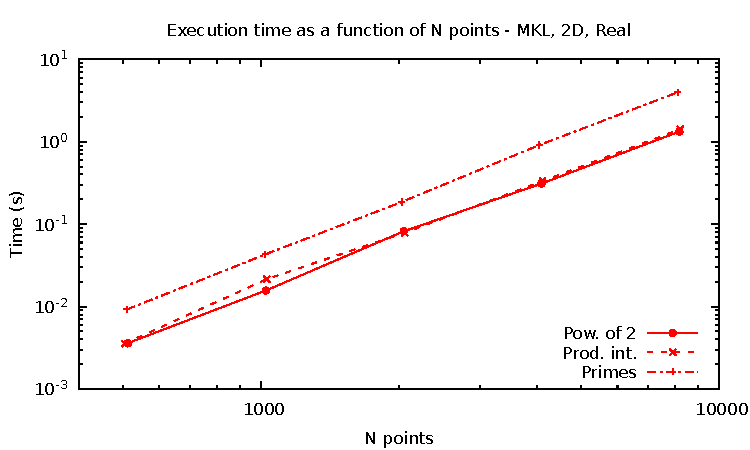
\includegraphics[width=.9\linewidth]{graphs/2d-mkl-exec-r.pdf}
\caption{Execution (real)}
\label{2DMKLR}
\end{subfigure}\\
\begin{subfigure}{.5\textwidth}
\centering
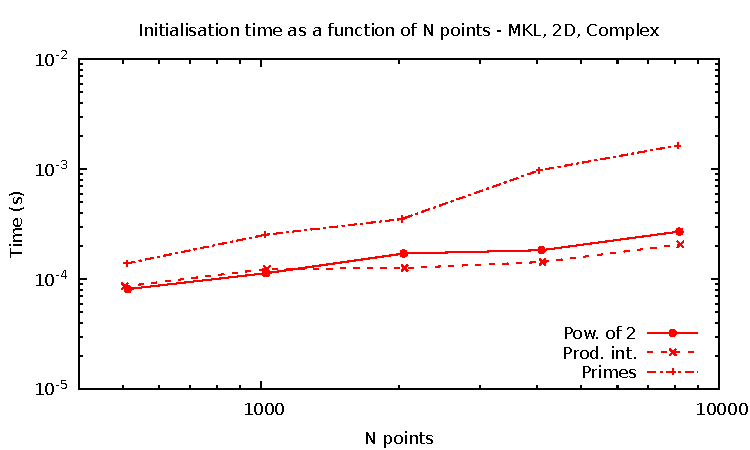
\includegraphics[width=.9\linewidth]{graphs/2d-mkl-init-c.pdf}
\caption{Intialisation (complex)}
\label{2DMKLCI}
\end{subfigure}%
\begin{subfigure}{.5\textwidth}
\centering
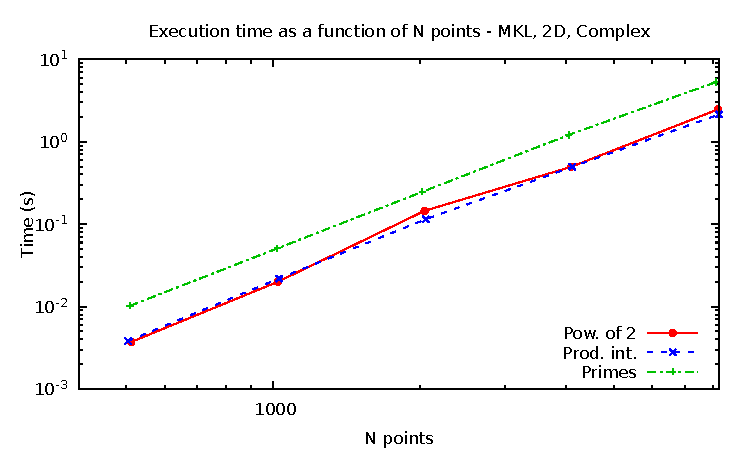
\includegraphics[width=.9\linewidth]{graphs/2d-mkl-exec-c.pdf}
\caption{Execution (complex)}
\label{2DMKLC}
\end{subfigure}
\caption{Initialisation and execution times as a function of the side of the square (2 dimensions, MKL)}
\label{2DMKL}
\end{figure}

\begin{figure}[H]
\captionsetup{width=0.8\linewidth}
\centering
\begin{subfigure}{.5\textwidth}
\centering
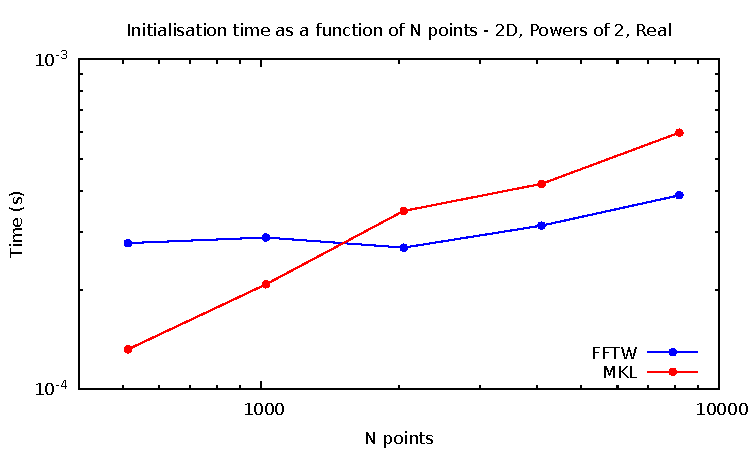
\includegraphics[width=.9\linewidth]{graphs/2d-pow2-init-r.pdf}
\caption{Intialisation (real)}
\label{2DPOW2RI}
\end{subfigure}%
\begin{subfigure}{.5\textwidth}
\centering
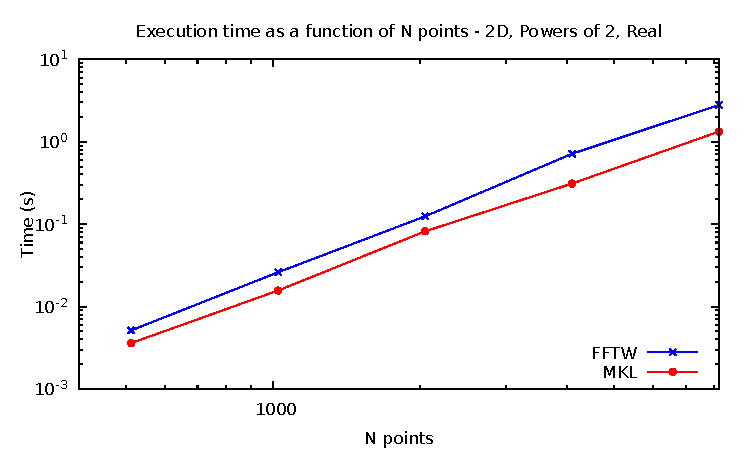
\includegraphics[width=.9\linewidth]{graphs/2d-pow2-exec-r.pdf}
\caption{Execution (real)}
\label{2DPOW2R}
\end{subfigure}\\
\begin{subfigure}{.5\textwidth}
\centering
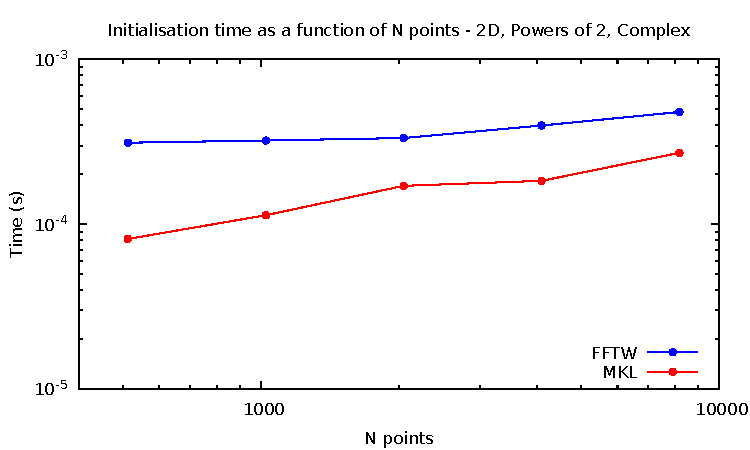
\includegraphics[width=.9\linewidth]{graphs/2d-pow2-init-c.pdf}
\caption{Intialisation (complex)}
\label{2DPOW2CI}
\end{subfigure}%
\begin{subfigure}{.5\textwidth}
\centering
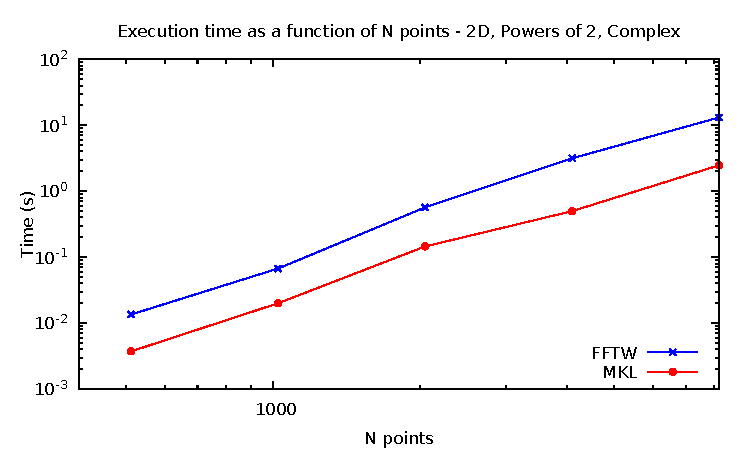
\includegraphics[width=.9\linewidth]{graphs/2d-pow2-exec-c.pdf}
\caption{Execution (complex)}
\label{2DPOW2C}
\end{subfigure}
\caption{Initialisation and execution times as a function of the side of the square (2 dimensions, powers of 2)}
\label{2DPOW2}
\end{figure}


\begin{figure}[H]
\captionsetup{width=0.8\linewidth}
\centering
\begin{subfigure}{.5\textwidth}
\centering
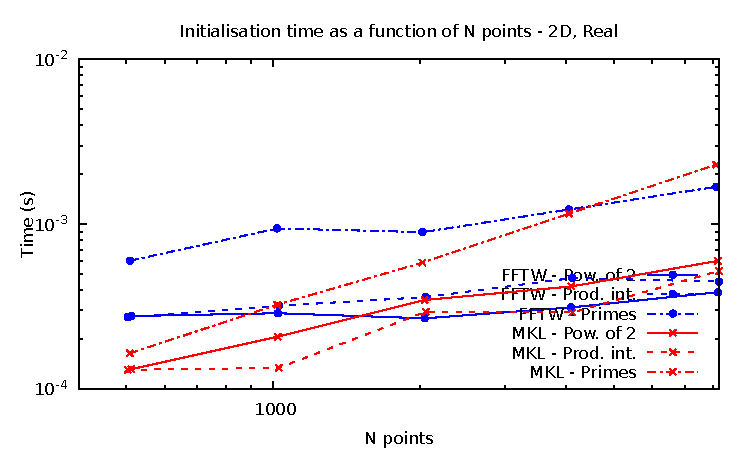
\includegraphics[width=.9\linewidth]{graphs/2d-init-r.pdf}
\caption{Intialisation (real)}
\label{2DRI}
\end{subfigure}%
\begin{subfigure}{.5\textwidth}
\centering
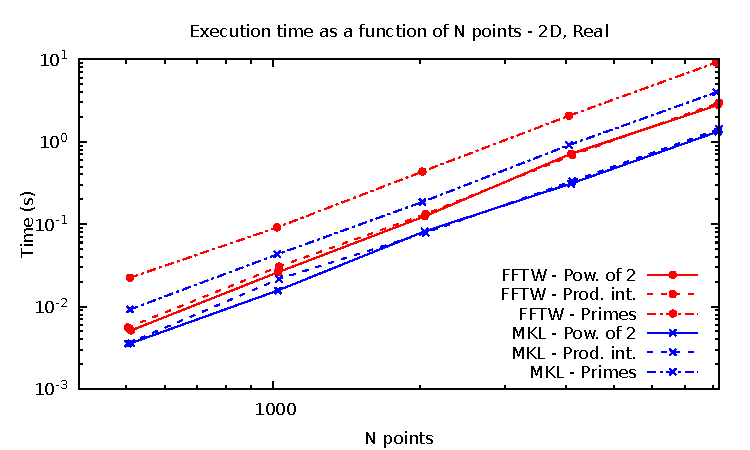
\includegraphics[width=.9\linewidth]{graphs/2d-exec-r.pdf}
\caption{Execution (real)}
\label{2DR}
\end{subfigure}\\
\begin{subfigure}{.5\textwidth}
\centering
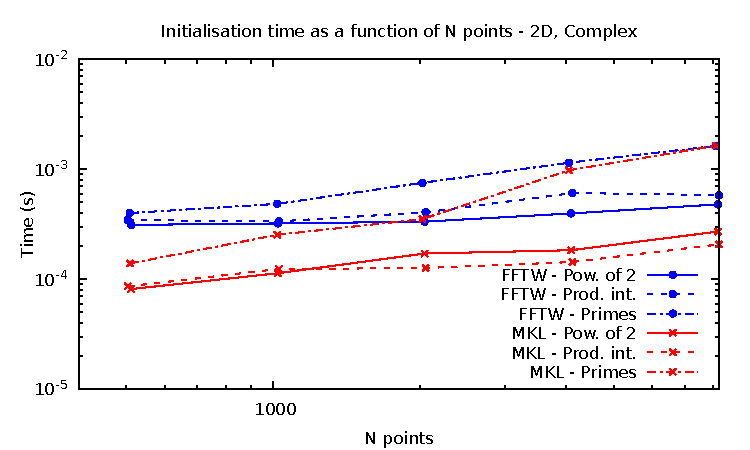
\includegraphics[width=.9\linewidth]{graphs/2d-init-c.pdf}
\caption{Intialisation (complex)}
\label{2DCI}
\end{subfigure}%
\begin{subfigure}{.5\textwidth}
\centering
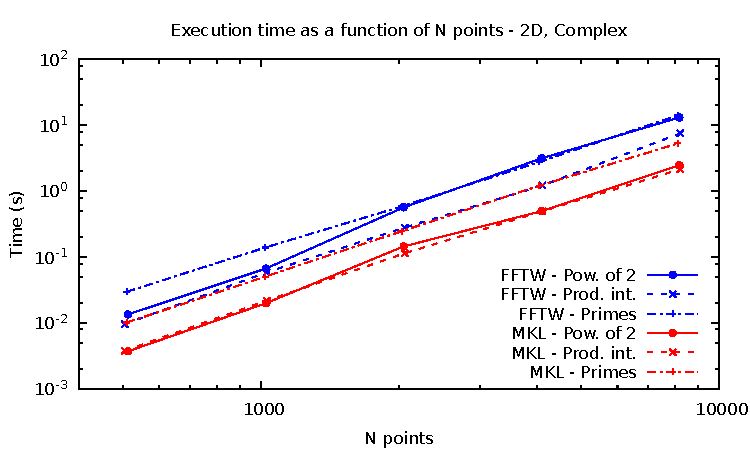
\includegraphics[width=.9\linewidth]{graphs/2d-exec-c.pdf}
\caption{Execution (complex)}
\label{2DC}
\end{subfigure}
\caption{Initialisation and execution times as a function of the side of the square (2 dimensions)}
\label{2D}
\end{figure}

\section{Effect of the domain size in three dimensions}\label{PERFORMANCE3D}

We repeat the analysis carried out in Sections \ref{PERFORMANCE1D} and \ref{PERFORMANCE2D} in three dimensions, on a cubic domain, with  the FFTW and MKL libraries. The number of points considered is given in Table \ref{SIZES3D}.

\begin{table}[H]
\captionsetup{width=0.85\linewidth}
\centering
\begin{tabular}{|l|l|l|}
  \hline
  \multicolumn{3}{|c|}{$N_x=N_y=N_z$}\\
  \hline
  \hline
  Powers of 2 & prod. pow. int. & primes\\ \hline
$2^5=32$ & $2\ 3\ 5=30$	& 31\\ \hline
$2^6=64$ & $2\ 5\ 7=70$	& 61\\ \hline
$2^7=128$ & $3\ 5\ 7=105$ & 127\\ \hline
$2^8=256$ & $2\ 3\ 5\ 7=210$ & 257\\ \hline
$2^9=512$ & $2^2\ 3\ 5\ 7=420$ & 509\\ \hline
\end{tabular}
\caption{Number of points on the side of the cube used for the benchmark}\label{SIZES3D}
\end{table}

As previously, the best performance is achieved when the number of points is a power of 2 or the product of powers of small integers rather than a prime number. We also observe that the MKL library is more efficient.
\begin{figure}[H]
\captionsetup{width=0.8\linewidth}
\centering
\begin{subfigure}{.5\textwidth}
\centering
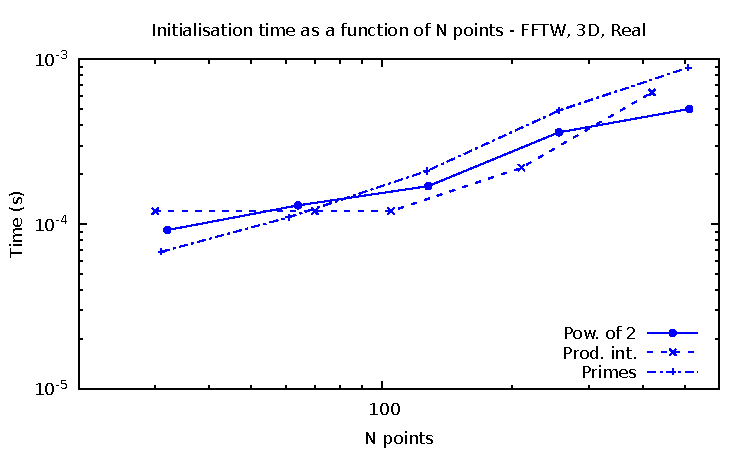
\includegraphics[width=.9\linewidth]{graphs/3d-fftw-init-r.pdf}
\caption{Intialisation (real)}
\label{3DFFTWRI}
\end{subfigure}%
\begin{subfigure}{.5\textwidth}
\centering
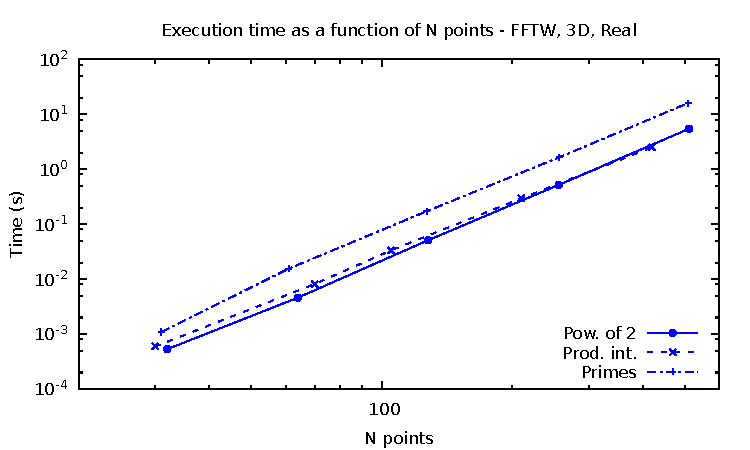
\includegraphics[width=.9\linewidth]{graphs/3d-fftw-exec-r.pdf}
\caption{Execution (real)}
\label{3DFFTWR}
\end{subfigure}\\
\begin{subfigure}{.5\textwidth}
\centering
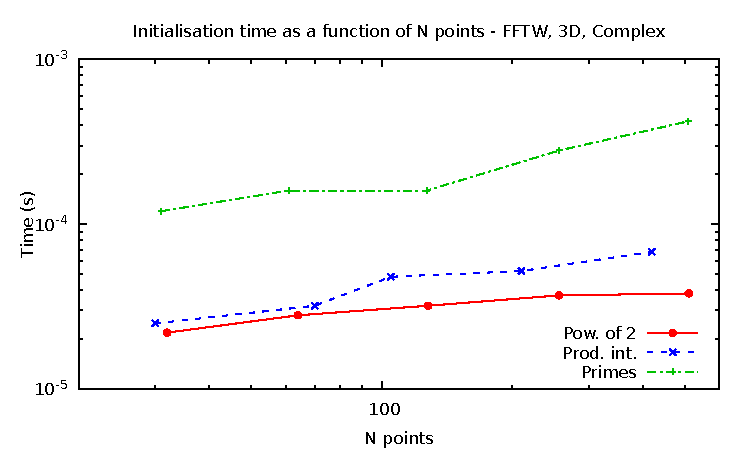
\includegraphics[width=.9\linewidth]{graphs/3d-fftw-init-c.pdf}
\caption{Intialisation (complex)}
\label{3DFFTWCI}
\end{subfigure}%
\begin{subfigure}{.5\textwidth}
\centering
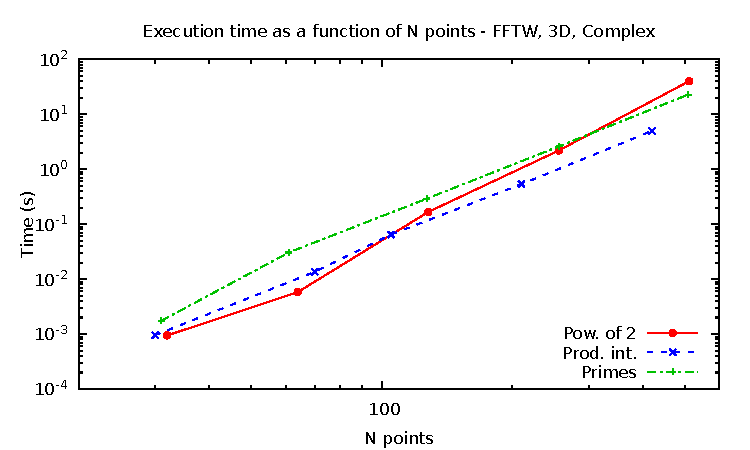
\includegraphics[width=.9\linewidth]{graphs/3d-fftw-exec-c.pdf}
\caption{Execution (complex)}
\label{3DFFTWC}
\end{subfigure}
\caption{Initialisation and execution times as a function of the side of the cube (3 dimensions, FFTW)}
\label{3DFFTW}
\end{figure}


\begin{figure}[H]
\captionsetup{width=0.8\linewidth}
\centering
\begin{subfigure}{.5\textwidth}
\centering
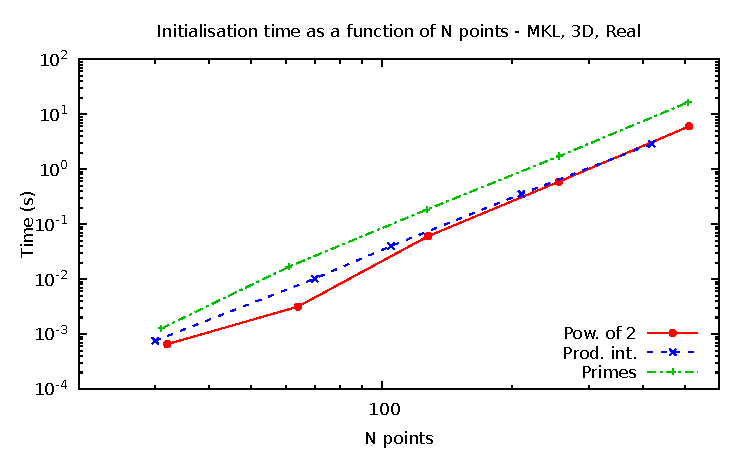
\includegraphics[width=.9\linewidth]{graphs/3d-mkl-init-r.pdf}
\caption{Intialisation (real)}
\label{3DMKLRI}
\end{subfigure}%
\begin{subfigure}{.5\textwidth}
\centering
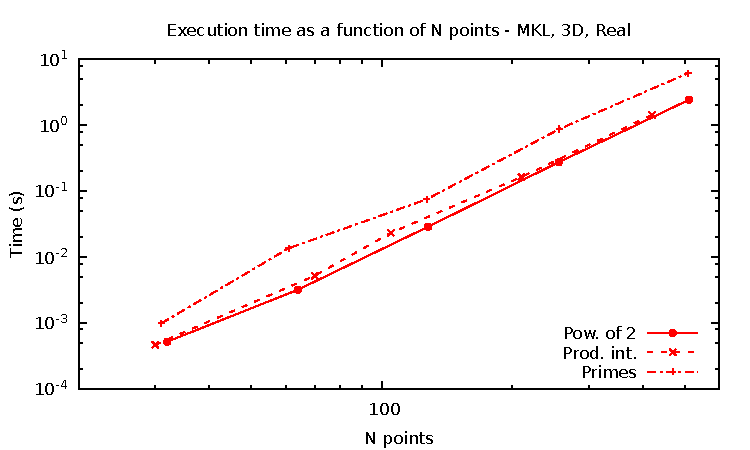
\includegraphics[width=.9\linewidth]{graphs/3d-mkl-exec-r.pdf}
\caption{Execution (real)}
\label{3DMKLR}
\end{subfigure}\\
\begin{subfigure}{.5\textwidth}
\centering
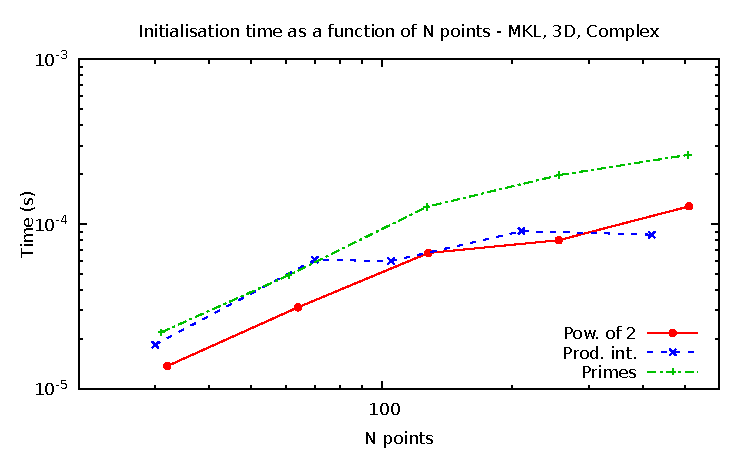
\includegraphics[width=.9\linewidth]{graphs/3d-mkl-init-c.pdf}
\caption{Intialisation (complex)}
\label{3DMKLCI}
\end{subfigure}%
\begin{subfigure}{.5\textwidth}
\centering
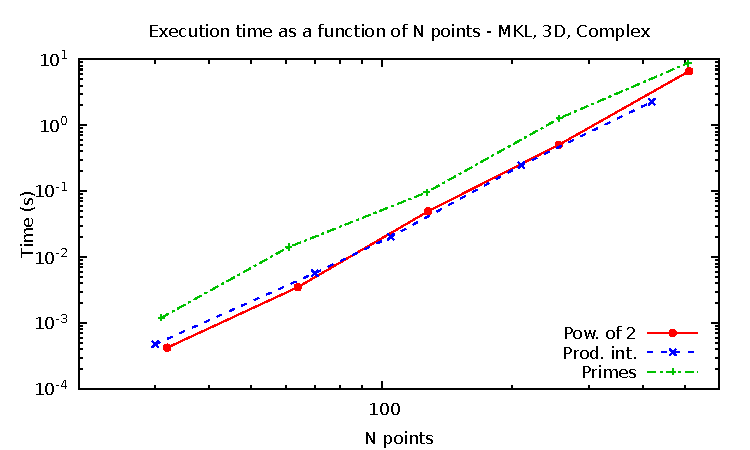
\includegraphics[width=.9\linewidth]{graphs/3d-mkl-exec-c.pdf}
\caption{Execution (complex)}
\label{3DMKLC}
\end{subfigure}
\caption{Initialisation and execution times as a function of the side of the cube (3 dimensions, MKL)}
\label{3DMKL}
\end{figure}

\begin{figure}[H]
\captionsetup{width=0.8\linewidth}
\centering
\begin{subfigure}{.5\textwidth}
\centering
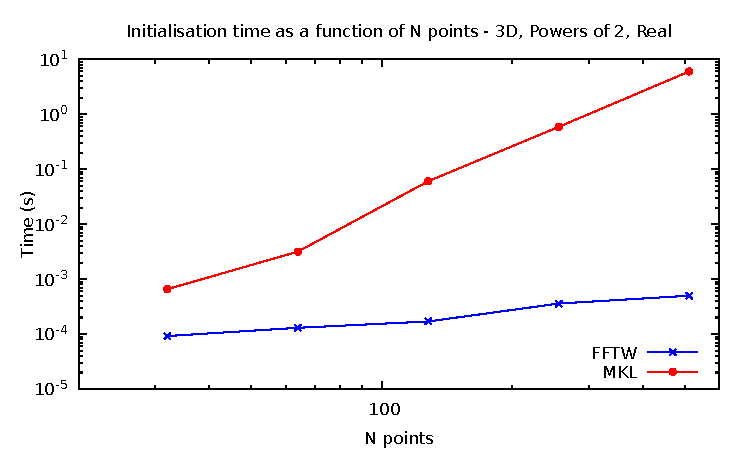
\includegraphics[width=.9\linewidth]{graphs/3d-pow2-init-r.pdf}
\caption{Intialisation (real)}
\label{3DPOW2RI}
\end{subfigure}%
\begin{subfigure}{.5\textwidth}
\centering
\includegraphics[width=.9\linewidth]{graphs/3d-pow2-exec-r.pdf}
\caption{Execution (real)}
\label{3DPOW2R}
\end{subfigure}\\
\begin{subfigure}{.5\textwidth}
\centering
\includegraphics[width=.9\linewidth]{graphs/3d-pow2-init-c.pdf}
\caption{Intialisation (complex)}
\label{3DPOW2CI}
\end{subfigure}%
\begin{subfigure}{.5\textwidth}
\centering
\includegraphics[width=.9\linewidth]{graphs/3d-pow2-exec-c.pdf}
\caption{Execution (complex)}
\label{3DPOW2C}
\end{subfigure}
\caption{Initialisation and execution times as a function of the side of the cube (3 dimensions, powers of 2)}
\label{3DPOW2}
\end{figure}

\begin{figure}[H]
\captionsetup{width=0.8\linewidth}
\centering
\begin{subfigure}{.5\textwidth}
\centering
\includegraphics[width=.9\linewidth]{graphs/3d-init-r.pdf}
\caption{Intialisation (real)}
\label{3DRI}
\end{subfigure}%
\begin{subfigure}{.5\textwidth}
\centering
\includegraphics[width=.9\linewidth]{graphs/3d-exec-r.pdf}
\caption{Execution (real)}
\label{3DR}
\end{subfigure}\\
\begin{subfigure}{.5\textwidth}
\centering
\includegraphics[width=.9\linewidth]{graphs/3d-init-c.pdf}
\caption{Intialisation (complex)}
\label{3DCI}
\end{subfigure}%
\begin{subfigure}{.5\textwidth}
\centering
\includegraphics[width=.9\linewidth]{graphs/3d-exec-c.pdf}
\caption{Execution (complex)}
\label{3DC}
\end{subfigure}
\caption{Initialisation and execution times as a function of the side of the cube (3 dimensions)}
\label{3D}
\end{figure}
\section{Effect of the flatness of the domain}\label{Sec:FLATNESS}

The experiments we carried out in Sections \ref{PERFORMANCE2D} and \ref{PERFORMANCE3D} were with domains whose dimensions were the same in all directions, that is, squares or cubes. In this section, we will study, in three dimensions, the effect of the flatness of the domain on the performance. We will compute the transform of a signal on a cuboid containing $512^3$ points stretched in the $z$ direction. The sides in the $x$ and $y$ directions have identical lengths ($N_x=N_y$) and the flatness is defined as the ratio between the number of points in the $z$ and $x$ directions ($N_z/N_x$). The dimensions of the domains considered appear in Table \ref{FLATNESSDIM}.
\begin{table}[H]
\centering
\begin{tabular}{|l|l|l|}
  \hline
  $N_x=N_y$ & $N_z $ & Flatness\\ 
  \hline
  \hline
512 & 512       & 1\\ \hline
256 & 2048      & 8\\ \hline
128 & 8192      & 64\\ \hline
64  & 32768     & 512\\ \hline
32  & 131072    & 4096\\ \hline
16  & 524288    & 32768\\ \hline
8   & 2097152   & 262144\\ \hline
4   & 8388608   & 2097152\\ \hline
2   & 33554432  & 16777216\\ \hline
1   & 134217728 & 134217728\\ \hline
\end{tabular}
\caption{Number of points used for the benchmark in three dimensions}\label{FLATNESSDIM}
\end{table}

We have observed that there is no clear trend in the way the flatness of the domain affects the performance and conclude that the performance depends mostly on the total number of points.

\begin{figure}[H]
\captionsetup{width=0.8\linewidth}
\centering
\begin{subfigure}{.5\textwidth}
\centering
\includegraphics[width=.9\linewidth]{graphs/flatness-r.pdf}
\caption{Real}
\label{FLATNESSR}
\end{subfigure}%
\begin{subfigure}{.5\textwidth}
\centering
\includegraphics[width=.9\linewidth]{graphs/flatness-c.pdf}
\caption{Complex}
\label{FLATNESSC}
\end{subfigure}
\caption{Execution time as a function of the flatness of the domain ($N_y/N_x$), for $N_y=N_z$ (3 dimensions, powers of 2)}
\label{FLATNESS}
\end{figure}

\section{Parallelism}\label{PARALLELISM}
So far, we have computed FFTs in a serial way. In this section, we will investigate the effect of parallelism on the performance achieved. Only the FFTW and MKL libraries are capable of running in parallel.  
\subsection{Multithreading}\label{MULTITHREADING}
We begin by considering the effect of multithreading on the computation of the transform of a cube of $512 \times 512 \times 512$ points. We carry out those measurements on a single node of ARCHER where we can use at most 24 threads. The MKL library is, once more, quicker. However FFTW scales a little better with the number of threads but it starts from  a lower performance.
\begin{figure}[H]
\captionsetup{width=0.8\linewidth}
\centering
\begin{subfigure}{.5\textwidth}
\centering
\includegraphics[width=.9\linewidth]{graphs/3d-multh-init-r.pdf}
\caption{Intialisation (real)}
\label{3DMULTHRI}
\end{subfigure}%
\begin{subfigure}{.5\textwidth}
\centering
\includegraphics[width=.9\linewidth]{graphs/3d-multh-exec-r.pdf}
\caption{Execution (real)}
\label{3DMULTHRE}
\end{subfigure}\\
\begin{subfigure}{.5\textwidth}
\centering
\includegraphics[width=.9\linewidth]{graphs/3d-multh-init-c.pdf}
\caption{Intialisation (complex)}
\label{3DMULTHCI}
\end{subfigure}%
\begin{subfigure}{.5\textwidth}
\centering
\includegraphics[width=.9\linewidth]{graphs/3d-multh-exec-c.pdf}
\caption{Execution (complex)}
\label{3DMULTHCR}
\end{subfigure}
\caption{Initialisation and execution times as a function of the number of threads (3 dimensions, $512 \times 512\times 512$ points, FFTW and MKL)}
\label{3DMKLMPITHREAD}
\end{figure}

\subsection{MPI}\label{MPI}
We now turn to studying the effect of the parallelism provided by MPI. In this case, we used up to 96 processes, corresponding to 4 ARCHER nodes, each with only a single thread. We carried out the measurements using a constant number of points on a line ($N_x=16777216$), a square ($N_x=N_y=4096$) and a cube ($N_x=N_y=N_z=256$). The MKL library is again more efficient, except in one dimension where it scales extremely poorly.
\begin{figure}[H]
\captionsetup{width=0.8\linewidth}
\centering
\begin{subfigure}{.5\textwidth}
\centering
\includegraphics[width=.9\linewidth]{graphs/mpi-init-1d.pdf}
\caption{Intialisation}
\label{1DMPII}
\end{subfigure}%
\begin{subfigure}{.5\textwidth}
\centering
\includegraphics[width=.9\linewidth]{graphs/mpi-exec-1d.pdf}
\caption{Execution}
\label{1DMPIE}
\end{subfigure}
\caption{Initialisation and execution times as a function of the number of processes (1 dimension)}
\label{1DMPI}
\end{figure}

\begin{figure}[H]
\captionsetup{width=0.8\linewidth}
\centering
\begin{subfigure}{.5\textwidth}
\centering
\includegraphics[width=.9\linewidth]{graphs/mpi-init-2d.pdf}
\caption{Intialisation}
\label{2DMPII}
\end{subfigure}%
\begin{subfigure}{.5\textwidth}
\centering
\includegraphics[width=.9\linewidth]{graphs/mpi-exec-2d.pdf}
\caption{Execution}
\label{2DMPIE}
\end{subfigure}
\caption{Initialisation and execution times as a function of the number of processes (2 dimensions)}
\label{2DMPI}
\end{figure}

\begin{figure}[H]
\captionsetup{width=0.8\linewidth}
\centering
\begin{subfigure}{.5\textwidth}
\centering
\includegraphics[width=.9\linewidth]{graphs/mpi-init-3d.pdf}
\caption{Intialisation}
\label{3DMPII}
\end{subfigure}%
\begin{subfigure}{.5\textwidth}
\centering
\includegraphics[width=.9\linewidth]{graphs/mpi-exec-3d.pdf}
\caption{Execution}
\label{3DMPIE}
\end{subfigure}
\caption{Initialisation and execution times as a function of the number of processes (3 dimensions)}
\label{3DMPI}
\end{figure}

\subsection{MPI and multithreading}\label{MPIMULTH}
We now combine multithreading with MPI in the same conditions as in Section \ref{MPI}. We increase the number of threads up to the number of cores on a compute node and subsequently increase the number of such processes. We carry out this procedure till we use 4 processes, each consisting of 24 threads. In one dimension\footnote{In one dimension, FFTW works in a distributed way only with a complex signal.}, the MKL library scales poorly and FFTW yields a better performance. In two dimensions, the MKL library is the fastest and the performance of FFTW improves only with several processes and not with multithreading. In three dimensions, only the MKL works and it does only with a single process. We conclude that, while multithreading and MPI bring a performance improvement separately, their combination leads to poor scaling and crashes. 
\begin{figure}[H]
\captionsetup{width=0.8\linewidth}
\centering
\begin{subfigure}{.5\textwidth}
\centering
\includegraphics[width=.9\linewidth]{graphs/mpi-multh-init-1d.pdf}
\caption{Intialisation}
\label{1DMPIMULTHI}
\end{subfigure}%
\begin{subfigure}{.5\textwidth}
\centering
\includegraphics[width=.9\linewidth]{graphs/mpi-multh-exec-1d.pdf}
\caption{Execution}
\label{1DMPIMULTHE}
\end{subfigure}
\caption{Initialisation and execution times as a function of the number of cores (1 dimension)}
\label{1DMPIMULTH}
\end{figure}

\begin{figure}[H]
\captionsetup{width=0.8\linewidth}
\centering
\begin{subfigure}{.5\textwidth}
\centering
\includegraphics[width=.9\linewidth]{graphs/mpi-multh-init-2d.pdf}
\caption{Intialisation}
\label{2DMPIMULTHI}
\end{subfigure}%
\begin{subfigure}{.5\textwidth}
\centering
\includegraphics[width=.9\linewidth]{graphs/mpi-multh-exec-2d.pdf}
\caption{Execution}
\label{2DMPIMULTHE}
\end{subfigure}
\caption{Initialisation and execution times as a function of the number of cores (2 dimensions)}
\label{2DMPIMULTH}
\end{figure}

\begin{figure}[H]
\captionsetup{width=0.8\linewidth}
\centering
\begin{subfigure}{.5\textwidth}
\centering
\includegraphics[width=.9\linewidth]{graphs/mpi-multh-init-3d.pdf}
\caption{Intialisation}
\label{3DMPIMULTHI}
\end{subfigure}%
\begin{subfigure}{.5\textwidth}
\centering
\includegraphics[width=.9\linewidth]{graphs/mpi-multh-exec-3d.pdf}
\caption{Execution}
\label{3DMPIMULTHE}
\end{subfigure}
\caption{Initialisation and execution times as a function of the number of cores (3 dimensions)}
\label{3DMPIMULTH}
\end{figure}

\subsection{Constant number of cores}\label{CONST}
We now compare the effects of multithreading and MPI by using a constant number of cores, 24, on a single node while varying the number of processes and threads. The signal is the same as in Sections \ref{MPI} and \ref{MPIMULTH}. As was stated in Section \ref{MPIMULTH}, multhreading, when combined with MPI, does not seem to yield a significant performance improvement. As a consequence, the performance improves only with an increasing number of threads. In one dimension, the MKL library scales poorly and FFTW gives the best performance. In two dimensions, the MKL library is the fastest. Finally, in three dimensions, we have only obtained data with the MKL library since FFTW crashes.
\begin{figure}[H]
\captionsetup{width=0.8\linewidth}
\centering
\begin{subfigure}{.5\textwidth}
\centering
\includegraphics[width=.9\linewidth]{graphs/const-init-1d.pdf}
\caption{Intialisation}
\label{1DCONSTI}
\end{subfigure}%
\begin{subfigure}{.5\textwidth}
\centering
\includegraphics[width=.9\linewidth]{graphs/const-exec-1d.pdf}
\caption{Execution}
\label{1DCONSTE}
\end{subfigure}
\caption{Initialisation and execution times as a function of the number of processes (1 dimension)}
\label{1DCONST}
\end{figure}

\begin{figure}[H]
\captionsetup{width=0.8\linewidth}
\centering
\begin{subfigure}{.5\textwidth}
\centering
\includegraphics[width=.9\linewidth]{graphs/const-init-2d.pdf}
\caption{Intialisation}
\label{2DCONSTI}
\end{subfigure}%
\begin{subfigure}{.5\textwidth}
\centering
\includegraphics[width=.9\linewidth]{graphs/const-exec-2d.pdf}
\caption{Execution}
\label{2DCONSTE}
\end{subfigure}
\caption{Initialisation and execution times as a function of the number of processes (2 dimensions)}
\label{2DCONST}
\end{figure}

\begin{figure}[H]
\captionsetup{width=0.8\linewidth}
\centering
\begin{subfigure}{.5\textwidth}
\centering
\includegraphics[width=.9\linewidth]{graphs/const-init-3d.pdf}
\caption{Intialisation}
\label{3DCONSTI}
\end{subfigure}%
\begin{subfigure}{.5\textwidth}
\centering
\includegraphics[width=.9\linewidth]{graphs/const-exec-3d.pdf}
\caption{Execution}
\label{3DCONSTE}
\end{subfigure}
\caption{Initialisation and execution times as a function of the number of processes (3 dimensions)}
\label{3DCONST}
\end{figure}

\section{Requirements from the CCP}\label{CCPPETMR}
We have also benchmarked the FFT libraries in a situation corresponding to a problem encountered by the CCP/PET-MR collaboration, by computing the transform of a series of 32 square complex images whose side consists of 256 points as well as the closest prime number (257) and product of powers of small integers ($2^2\ 3^2\ 7=252$). We have repeated the algorithm described in Table \ref{PSEUDOCODE} but, this time, with $N_s=32$. In this case, the MKL library performs better than FFTW. None of the other libraries we have considered could be used in two dimensions. GSL works only in one dimension. The FORTRAN version of FFTPACK does not share that limitation. However all the C/C++ wrappers we have found offer only one-dimensional transforms. Finally FFTPACK is distributed with a licence that is less constraining than the GPL but, nevertheless, the C++ wrapper provided by CASA that we have used is distributed under the GPL v2.

\begin{figure}[H]
\captionsetup{width=0.6\textwidth}
\centering
\includegraphics[height=8cm]{graphs/ccppetmr.pdf}
\caption{Execution time for the transform of 32 complex square images as a function of square side\\(2 dimensions, complex)}
\label{method}
\end{figure}
\section{Conclusion}
When the FFT is executed serially, in one dimension, the situation is not very clear but FFTW seems to be the most efficient. In two and three dimensions, the MKL library is the fastest. When run in parallel with MPI or multithreading separately, the MKL library also performs best, except in one dimension. Finally, combining MPI with multithreading leads, in our experiments, to problems such as poor scaling and crashes.  
\section{Acknowledgements}
The special sentence that only Barbara knows.
\begin{thebibliography}{9}

\bibitem{CT}
Cooley J. W., Tukey J. W.
{\it An algorithm for the machine calculation of complex Fourier series},
Math. Comp. 19 (1965), 297-301
 
\bibitem{fftw}
Frigo, Matteo and Johnson, Steven G.,
{\it The Design and Implementation of FFTW3},
Proceedings of the IEEE,
2005,
93,
2,
216--231,
Special issue on ``Program Generation, Optimization, and Platform Adaptation''
\bibitem{mkl}
\url{https://software.intel.com/en-us/mkl}

\bibitem{gsl}
M. Galassi et al, {\it GNU Scientific Library Reference Manual (3rd Ed.)}, ISBN 0954612078
  
\bibitem{fftpack}
P.N. Swarztrauber, {\it Vectorizing the FFTs}, Parallel Computations (G. Rodrigue, ed.), Academic Press, 1982, pp. 51--83.
  
\bibitem{casa}
McMullin J. P., Waters B., Schiebel D., Young W., Golap K.,
{\it Astronomical Data Analysis Software and Systems XVI},
ASP Conf. Ser. 376, ed. R. A. Shaw, F. Hill, D. J. Bell (San Francisco, CA: ASP), 127

\bibitem{code}
\url{https://github.com/SoftwareOutlook/FFTC}
    
\bibitem{ccppetmr}
\url{https://www.ccppetmr.ac.uk/}

\bibitem{softwareoutlook}
Software Outlook \url{https://www.softwareoutlook.ac.uk/}

\bibitem{archer}
ARCHER is the UK National Computing Service (\url{https://www.archer.ac.uk/})
  
\end{thebibliography}

\end{document}
